  {\large \fontB Description:}
  
  {\bf solS} is a 2-dimensional analytical solution to the Cauchy equations with the acceleration term set to zero to represent creeping flow. The domain is given by $\Omega = [0,1] \times [0,1]$.
  The flow is driven by the velocity field
  \begin{equation}
    \boldsymbol v = \sin (n \pi x ) \boldsymbol i,
    \qquad \mbox{on $y = 1$}.
  \end{equation}
  applied on the upper horizontal boundary. No body forces are present so $\boldsymbol f = \boldsymbol 0$.
  The boundary conditions on the remaining walls are free-slip on the vertical sides and no slip on the lower horizontal boundary. 
  The viscosity is set to 1.0.

 {\large \fontB Parameters:}
  
 The variable parameters of this solution are:
 \begin{itemize}
   \item{wave number in x domain: $n \in \mathbb{Z} \medspace \backslash \medspace \{0\}$.}
 \end{itemize}

%  \begin{SCfigure}[][h]
%    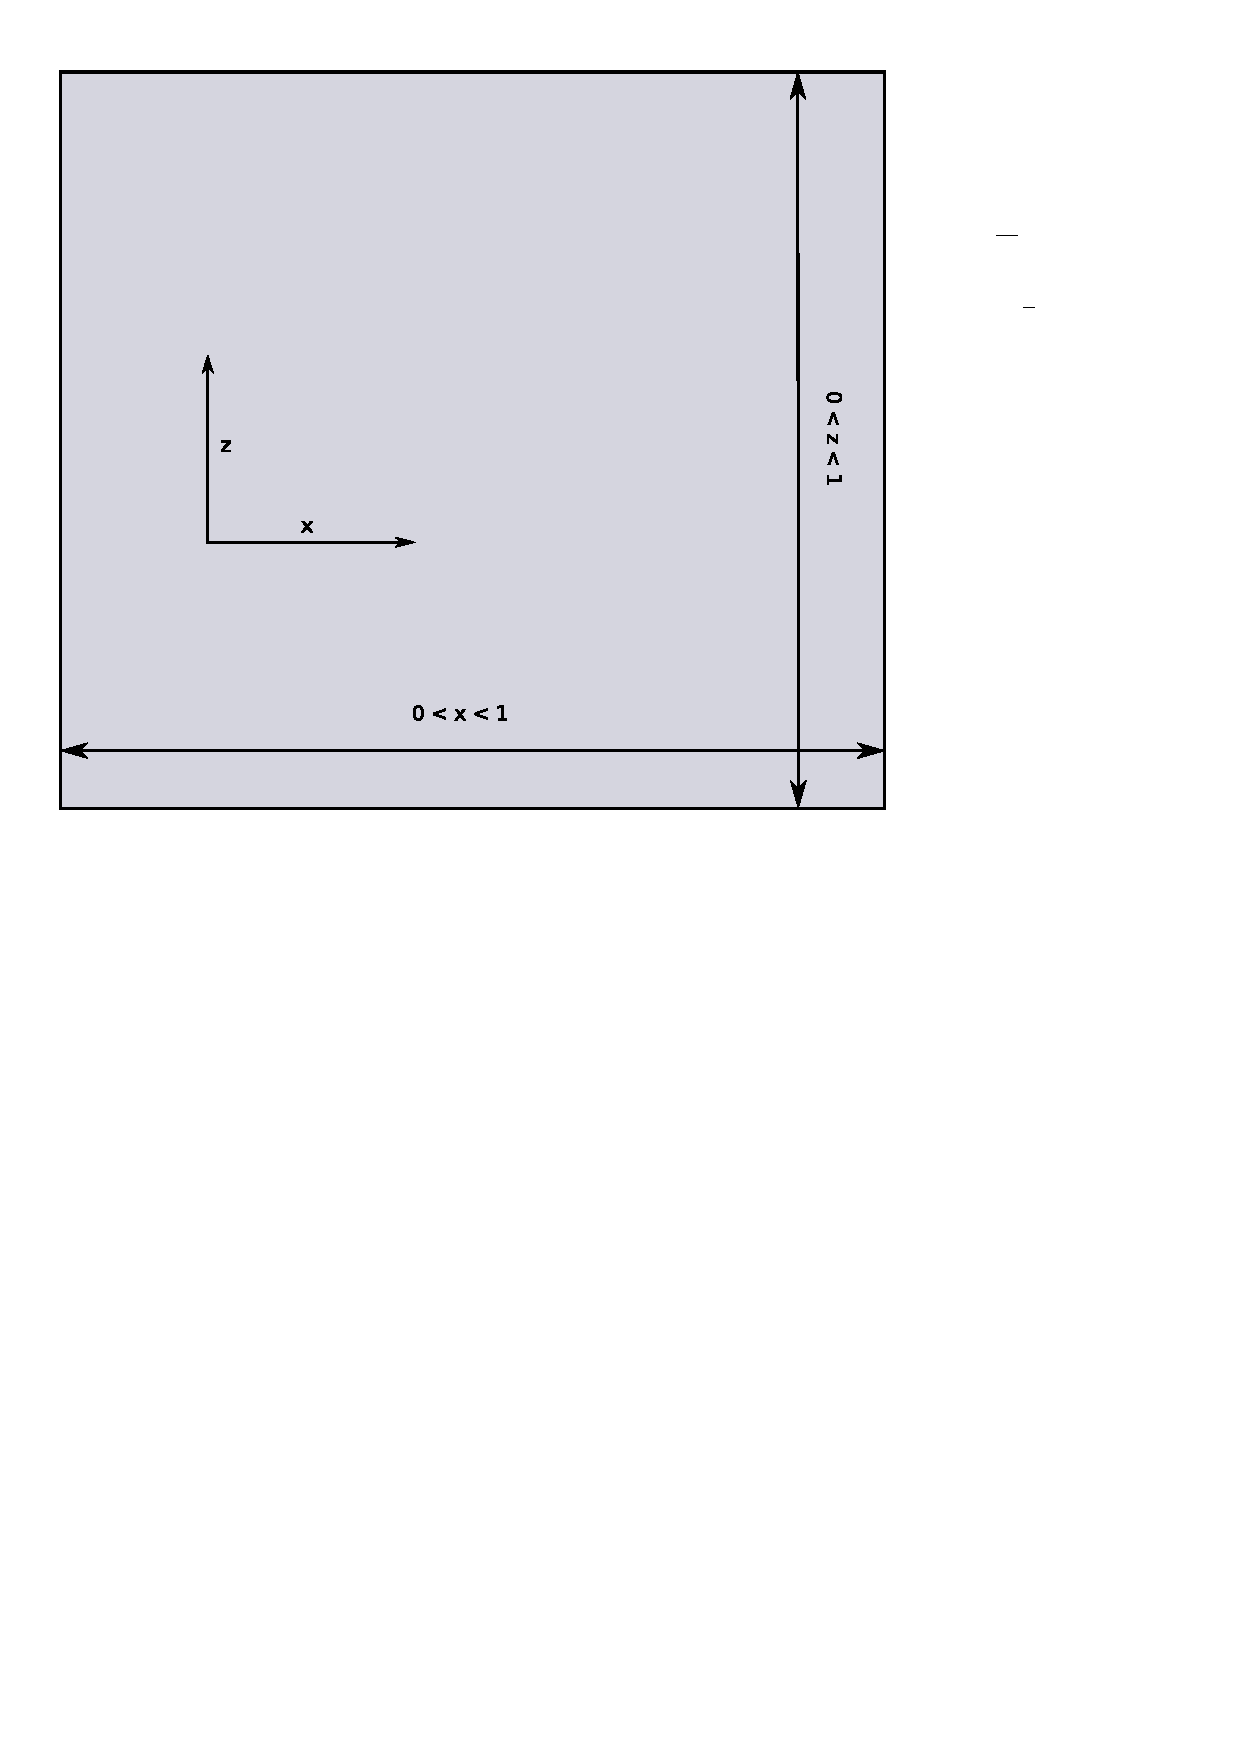
\includegraphics[width=6cm,clip]{../figs/figA}
%    \caption[Short caption]{\label{figA} 
%      Solution ({\bf SolA}):
%      This solution has a box of density $\rho = -\sigma \sin (k_m z) \cos (k_n x)$ .
%      It is isoviscous.
%      The Boundary conditions are free slip everywhere on the surfaces of the unit box.}
%  \end{SCfigure} 
%  \vspace{-47mm}
%  {\small
%  \[
%    \hspace{-77mm} \rho = -\sigma \sin (k_m z) \cos (k_n x)
%  \]
%  }
%  \vspace{47mm}
  
 {\large \fontB Solution:}
This problem has a simple analytic solution and is thus provided here:
\begin{align}
	v_x &= \sin( n \pi x ) 
		\Bigl( 
			( A n \pi + C + C n \pi y) \exp( n \pi y ) 
			- ( B n \pi - D + D n \pi y ) \exp( - n \pi y )
		 \Bigr)	\\
%
	v_y &= - n \pi \cos( n \pi x )
		\Bigl( 
  			( A + C y ) \exp( n \pi y ) 
			+ ( B + D y ) \exp( - n \pi y ) 
		\Bigr)	\\
%
	p &= - 2 n \pi \cos( n \pi x ) \Bigl( C \exp( n \pi y ) + D \exp( - n \pi y ) \Bigr)
\end{align}

The strain rate and deviatoric stress can be assembled from the velocity gradients given below; 
\begin{align}
	\frac{\partial v_x}{\partial x} 
	&= n \pi \cos(n \pi x) \Bigl( 
			( A n \pi + C + C n \pi y) \exp(n \pi y) 
			- ( B n \pi - D + D n \pi y) \exp(-n \pi y) 
			\Bigr)	\\
%
	\frac{\partial v_y}{\partial x} 
	&= n^2 \pi^2 \sin(n \pi x) \Bigl( 
		( A + C y ) \exp(n \pi y) 
		+ ( B + D y ) \exp(-n \pi y) 
		\Bigr)	\\
%
	\frac{\partial v_x}{\partial y} 
	&= \sin(n \pi x) \Bigl( 
		( A n^2 \pi^2 + 2 C n \pi + C n^2 \pi^2 y ) \exp(n \pi y) 
		+ ( B n^2 \pi^2 - 2 D n \pi + D n^2 \pi^2 y ) \exp(-n \pi y) 
		\Bigr)	\\
%
	\frac{\partial v_y}{\partial y} 
	&= - n \pi \cos(n \pi x) \Bigl( 
		( A n \pi + C + C n \pi y ) \exp(n \pi y) 
		+ ( -B n \pi + D - D n \pi y ) \exp(-n \pi y) 
		\Bigr)	\\
\end{align}


The constants $A, B, C, D$ and $E$ are given by
\begin{align}
	E &= (4 n^2 \pi^2 + 2 ) \exp^2( n \pi ) - \exp^4( n \pi ) - 1	\\
%	
	A &=  \frac{1}{E} ( \exp^2( n \pi ) - 1 ) \exp( n \pi )	\\
	B &= - A	\\
%	
	C &=   \frac{1}{E} \Bigl( 2 n \pi - \exp^2( n \pi ) + 1 \Bigr) \exp( n \pi )	\\
	D &= - \frac{1}{E} \Bigl(  2 n \pi \exp^2( n \pi ) - \exp^2( n \pi ) + 1 \Bigr) \exp( n \pi )
\end{align}









